\documentclass[a4paper,ngerman]{scrartcl}

\usepackage{amsmath}
\usepackage{amsfonts}
\usepackage{amssymb}
\usepackage[utf8]{inputenc}
\usepackage{graphicx}
\usepackage[ngerman]{babel}
\usepackage{hyperref}
\usepackage{float}
\usepackage{caption}
\usepackage{subcaption}
\usepackage{multirow}  %for tables
\usepackage{icomma} % Handle german comma as decimal point in numbers
\usepackage{units,siunitx} % Write units with correct spacing
\usepackage{upgreek} % provide non-italic greek letters
\usepackage{url}
%\usepackage{subfig}

% Formatting of table & figure captions
\captionsetup{font={sf,footnotesize},labelfont=bf,skip=6pt}
\setlength{\abovecaptionskip}{6pt}
\setlength{\belowcaptionskip}{0pt}

\title{Black Lipid Membrane\\ Auswertung}
\date{\today}
\author{Michel Rausch, Michael Eliachevitch}

\begin{document}

\maketitle
\tableofcontents
\newpage

\section{Aufgabe 1: Vorbereitung der Lipidmembran}

\begin{figure}[tbh!]
  \centering
  \includegraphics[width=.4\textwidth]{abbildungen/ohnelipidschicht_cut.jpg}
  \caption{"`Loch"' ohne Lipidschicht. Es befindet sich am Ende eines Rörchens, dass den inneren und äußeren Teil der Küvette verbindet.
Es erscheint schwarz, da daran kein Licht reflektiert wird.\\
Die Kreisrunde Reflexion am Rand indiziert, dass die Lichtquelle richtig eingestellt ist, um Newtonsche Ringe beim Anbringen einer
Lipidschicht zu sehen. Die folgenden Bilder der Lipidschicht sind so ausgeschnitten, dass der äußere Rand nicht mehr sichtbar ist und man nur den inneren Rand des Lochs sieht.}
  \label{fig:loch}
\end{figure}

\begin{figure}[tbh!]
  \centering
  \includegraphics[width=.4\textwidth]{abbildungen/newton2_cut.jpg}
  \caption{"`Loch"' mit angebrachter Lipidschicht. Sie ist schon dünn genug, dass man Newtonsche Ringe sieht, da die Dicke im Bereich der Wellenlänge ist. Am unteren Rand ist als schwarzer Fleck die BLM zu sehen, die sich gerade herausbildet und in der Lididschicht ausbreitet.
Sie ist nun noch dünner, sodass es zu keiner Interferenz zu Newtonschen Ringen mehr kommt, weshalb sie schwarz erscheint.}
  \label{fig:loch}
\end{figure}

\begin{figure}[tbh!]
  \centering
  \begin{minipage}[b]{.4\textwidth}
    \includegraphics[width=1.\textwidth]{abbildungen/lipid5final_cut.jpg}
  \end{minipage}
  \begin{minipage}[b]{.4\textwidth}
    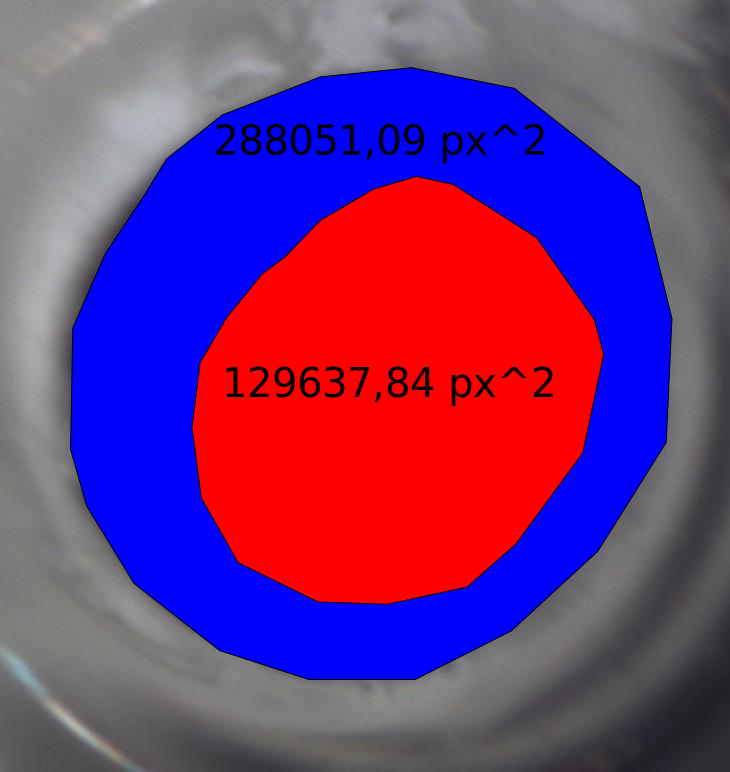
\includegraphics[width=1.\textwidth]{abbildungen/flaechenbestimmung.pdf}
  \end{minipage}
  \caption{Links ist eine vollständig ausgebildete BLM innerhalb des Lochs zu sehen.
Es ist bekannt, dass das Loch einen Durchmesser von 1\,mm. Durch Verhältnisbildung kann damit die Fläche 
der BLM bestimmt werden. Die Flächen auf dem Bilden hätten durch Bestimmung der Durchmesser abgeschätzt werden können. Da die BLM jedoch
nicht kreisförmig ist, haben wir die beiden relativen Fläche bestimmt, indem wir in dem Vektorgrafik-Programm "`Inkscape"'
jeweils um den Rand des Lochs und um die BLM Polygonpfade gelegt haben und die darin eingeschlossenen Flächen berechnen lassen haben. Die so 
berechneten relativen Flächen sind rechts zu sehen.\\
Daraus folgt, dass die BLM etwa 45\% des Lochs bedeckt, was bei einem Lochdurchmesser von 1\,mm einer Fläche von 0.353\,mm~$^2$ entspricht.}
\end{figure}

\section{Aufgabe 2: Messung einzelner Ionenkanäle}

\section{Aufgabe 3: Messung multipler Ionenkanäle}

\section{Aufgabe 4: Weitere Fragen}

\section{Quellen}
\begin{enumerate}
\item Vorbereitungsmappe 
\end{enumerate}



\end{document}
